\chapter{Generative Adversarial Networks (GAN)}

\section{Introduction}
Till now we have focused our attention on \textit{discriminative models} that roughly speaking, given some data in a given space $x$, gives by a certain \textit{probability distribution} the information on which class $y$ they are part. There are plenty of machine learning techniques that solve effectively this type of task. These models are seeking in \underline{existing data} some interesting patterns and use them in order to predict a class (classification) or a continuous number (regression).\\
At the opposite \textbf{generative models} given a noise input $z$ and a certain class $y$, generate a new, never seen sample $x$ for that class. In this chapter, in particular we are going to talk about \textit{GANs (Generative Adversarial Networks)} which were invented by a PhD student (Ian Goodfellow), this enabled computers in the generation of new data using not one, but \textbf{two different neural networks}. 

\begin{figure}[h]
    \centering
    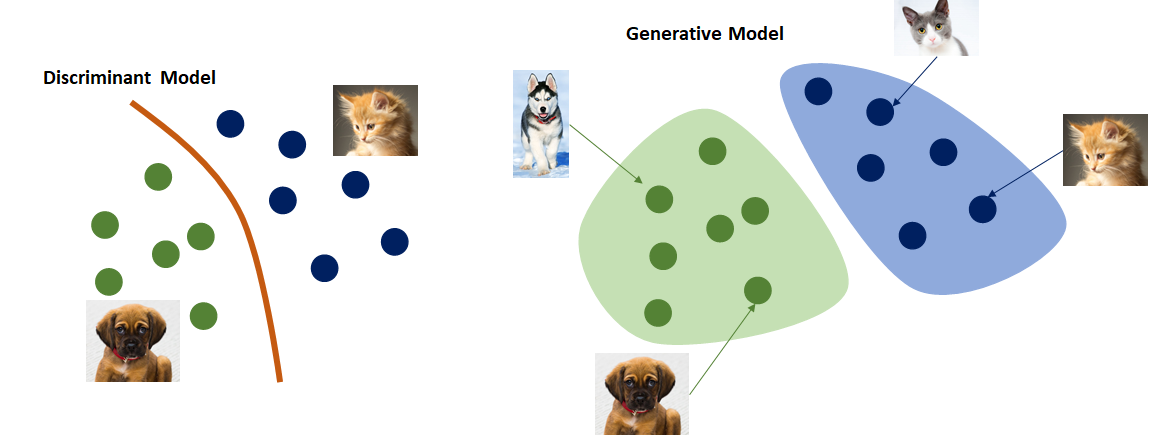
\includegraphics[scale=0.3]{img/generative_1.png}
    \caption{Discriminative vs Generative Models}
\end{figure}

\section{Variational Auto-Encoders (VAE)}
We consider here as a first approach to generative models the \textbf{autoencoders} and \textbf{variational autoencoders}, for several reasons: (i) it is an easier setting for generative AI; (ii) since generative models are challenging to be understood, autoencoders are closer to the models we have already seen, (iii) the autoencoders are directly or implicitly used in some variants of GAN architectures.

\subsection{Autoencoders}
The structure of an autoencoder is quite intuitive and follows these few steps: 
\begin{enumerate}
    \itemsep-0.3em
    \item \textsc{Encoder Network} this is the stage where we take a (full) representation $x$ (of an image for example) and reduce its dimension into a space $z$ by using a \underline{learned} encoder (a  classical ConvNet for example); 
    \item \textsc{Latent space} this is an intermediate stage in which the autoencoder architecture tidies its \textit{thoughts}; 
    \item \textsc{Decoder Network} we reconstruct the original dimension of the input $x$, starting from the latent space into a new generated image we call $x^*$.
\end{enumerate}

\begin{figure}
    \centering
    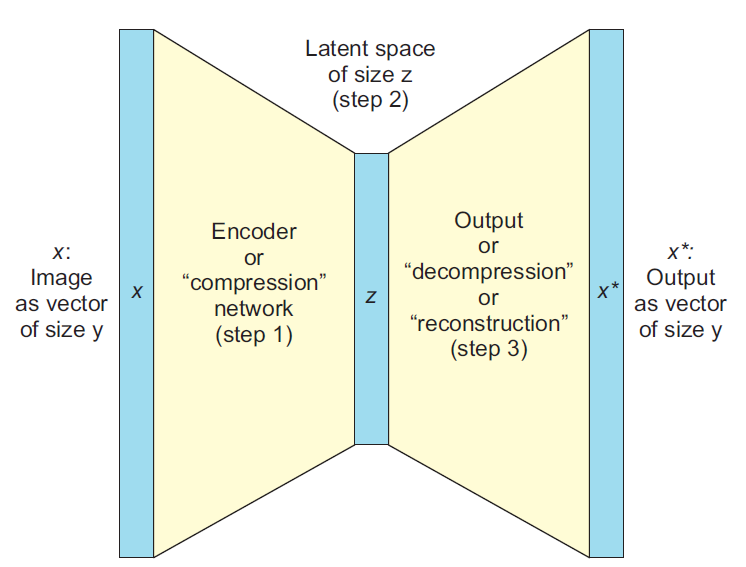
\includegraphics[scale=0.5]{img/autoencoder.png}
    \caption{Autoencoder architecture}
\end{figure}

\noindent
The \textit{training of an autoencoder} occurs as follows: 
\begin{enumerate}
    \itemsep-0.3em 
    \item We take the images $x$ through the autoencoder; 
    \item We collect the generated images $x^*$ as reconstruction of the given images;
    \item We measure a form of \textit{reconstruction loss} by mean (for example) of a mean squate error between the pixels of $x$ and $x^*$
    \item We obtain an explicit objective function to be minimized by mean of a gradient descent approach:
    \begin{equation}
        \mathcal{L}=\Vert x-x^* \Vert_2^2 
    \end{equation}
\end{enumerate}
The autoencoders can work by mean of an unsupervised machine learning model where we learn only from the training data without the labels. Note that we have a single loss function to be optimized with the common goal of \textit{minimizing the differences between the input and output images}.
We can use an autoencoder for different purposes, for example: image denoising, image colorization... 

\subsection{Variational autoencoders}
The traditional autoencoder maps the features of the input space into a latent space where the representation $z$ is nothing but a set of numbers. The main difference between autoencoders and Variational autoencoders (VAE) is just on the "magic" latent space. In fact here the choice is to represent the latent space as a \textit{probability distribution} with a certain mean ($\mu$) and a standard deviation $(\sigma)$. Note that you have to learn such a distribution! Once you have the distribution, you sample some numbers from it, add some noise and feed them to the decoder that will generate something that looks like the images of the training set, with the only difference they are \textbf{newly generated}. 

\begin{figure}[h]
    \centering
    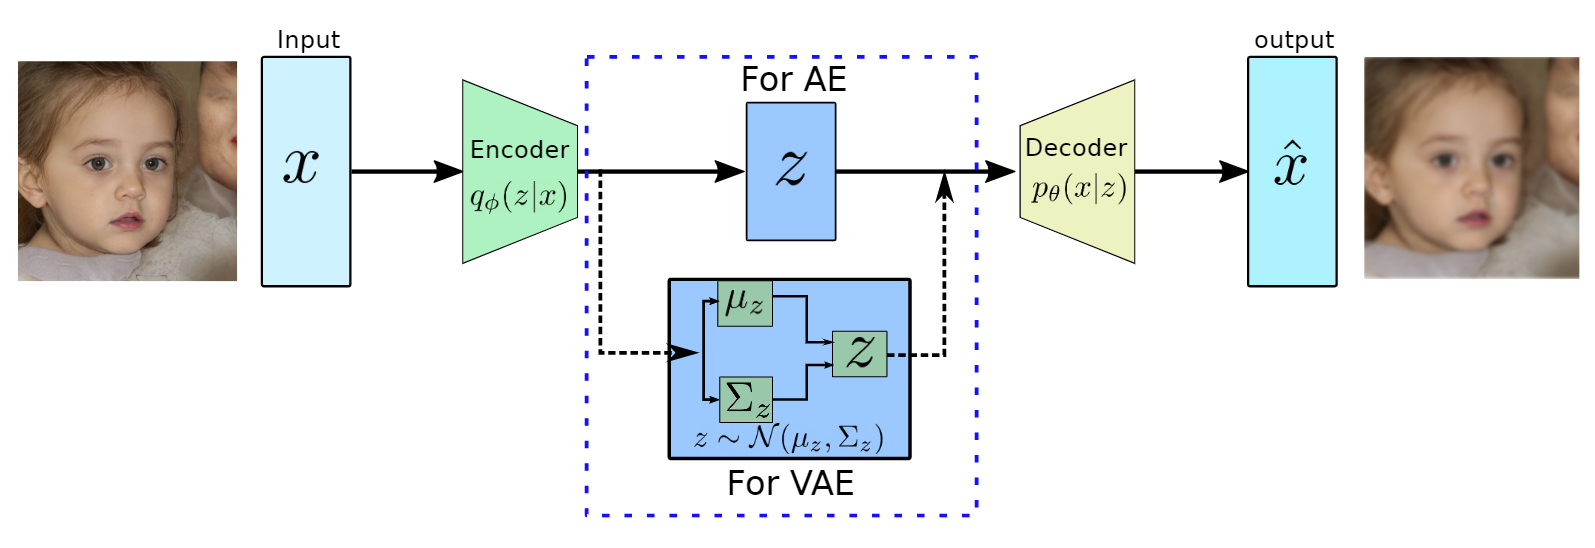
\includegraphics[scale=0.7]{img/VAE.png}
    \caption{(Variational) Auto-Encoder}
\end{figure}

\section{Generative Adversarial Networks}
\textbf{\textit{Generative Adversarial Networks} (GANs)} constitute a class of machine learning techniques which consist of two jointly trained models: the first (the \textit{Generator}) trained to create (generate) fake data, and the other (the \textit{Discriminator}) trained to binary distinguish fake data from real data. Let us go more deeply in the description of the GAN term:
\begin{description}
    \item[GENERATIVE] is the overall purpose of the machine learning model: generate new data. Clearly the generated data (images for example) depends on the features of the training set. If we want to generated new pictures of Leonardo Da Vinci, we must have a training set with Leonardo Da Vinci's portrait.
    \item[ADVERSARIAL] term refers to the game-like, competitive dynamic between the two models that constitute such a framework: the Generator and the Discriminator. The form is like an \textit{art forgery} while the discriminator is like an \textit{art expert} whose role is to say wheter a painting is fake or real; 
    \item[NETWORK] the models used for representing the two counterpart of the architecturesare neural networks. According to the complexity of the model, these can be simply Fully Connected Network, or ConvNet or in even more complex cases architectures like U-Net.   
\end{description}

This vanilla architecture is not suitable when: 
\begin{enumerate}
    \item We have large variations and different classes, while it performs well with small variations and small datasets;
    \item In such a type of architecture there is no way to control what the network have to generate.
\end{enumerate}
Both these issues are addressed introducing some novel aspects in the basic architecture, how we will see in the next sections.\\
Nowadays, GANs are used in order to synthetize artificially some images of some class or for other purposes like text to image or image to image translation. It is remarkable that for GAN there is not a latent space that will be decoded into a generated sample, due to the presence of a discriminator that allows the generator to be improved.

\begin{figure} 
    \centering
    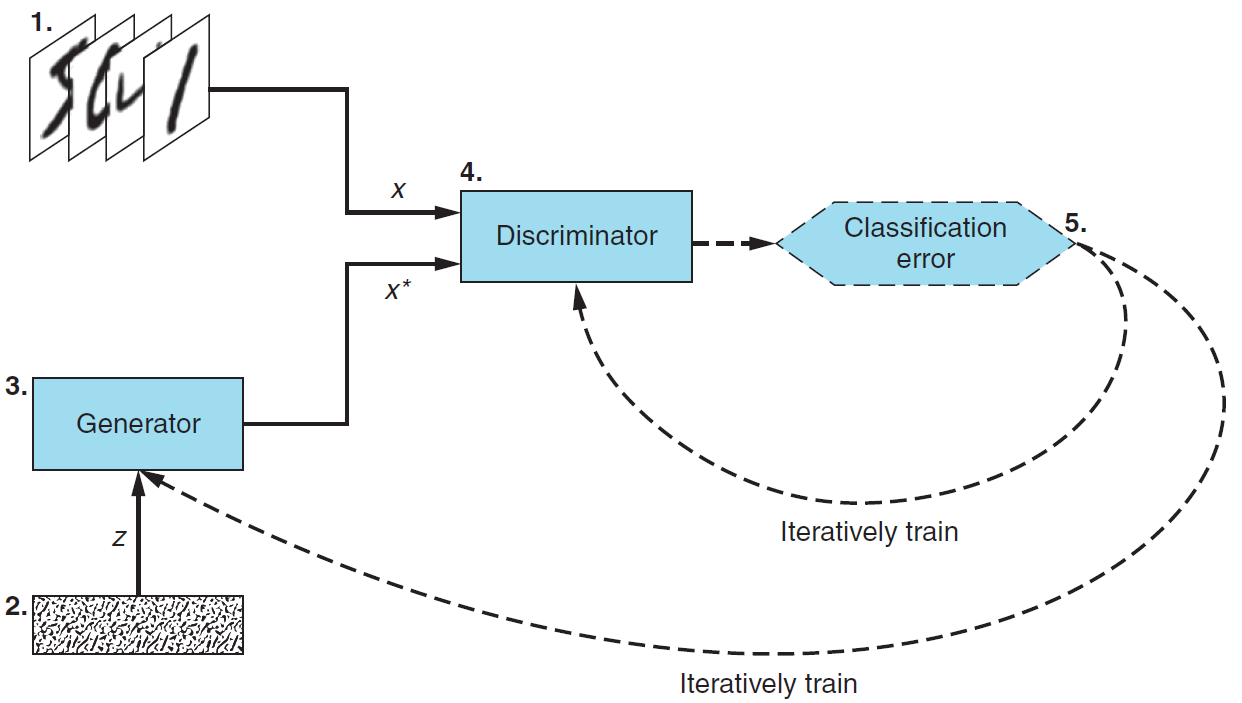
\includegraphics[scale=0.6]{img/GAN_1.png}
    \caption{GAN architecture}
    \label{fig:GAN_arch}
\end{figure}

\subsection{GAN anatomy}
The \Cref{fig:GAN_arch} shows the architecture of a GAN in its original form. Let us analyze the details of such diagram: 
\begin{enumerate}
    \itemsep-0.2em
    \item \textit{Training dataset} these are the real examples from which we want to learn the features, this is the input $x$ to the discriminator network
    \item \textit{Random noise vector} Is the input $z$ of the Generator network, is nothing but a vector of random number that the generating network uses as a starting point;
    \item \textit{Generator network} Takes as input the noise vector $z$ and outputs fake samples $x^*$, its goal is to produce samples that are as close as possible to the real data in order to fool  the Discriminator; 
    \item \textit{Discriminator network}  takes as input either a real example $x$ or a fake one $x^*$, for each generated example the Discriminator determines and outputs the probability of wheter an example is real/fake.
    \item \textit{Iterative training tuning} where the Discriminator's weights and biases are update in order to maximize the classification accuracy (maximizing the probability that $x \to${real} and $x^* \to$ fake), while the Generator's weights and biases are updated in order to maximize the probability that the discriminator classify $x^*$ is real. This is the reason why the two networks are as in a competition.
\end{enumerate}
Now we can say that: (i) at the end of the training the discriminator models $p(y|x)$ where $y$ can be real or fake; (ii) the generator learns a certain probability $p(x|y)$ that depends on the characteristics of the training set, that is the most common examples in the training set will be the most likely to be generated.\\

Note that the discriminator is used only in training phase: once you have obtained the learned generator, it is sufficient to provide it some noise vectors that will be mapped into generated images.

\subsection{Training GAN}
Till now we have done a snapshot of the engine analyzing the main features and the components it is made up of. An explanation of the training process is given here in order to better understand the mechanisms under the hood. The training of a GAN sees the alternate tuning of the Discriminator and Generator. In particular: 
\begin{enumerate}
    \itemsep-0.3em
    \item \textsf{Train the Discriminator}
    \begin{itemize}
        \itemsep-0.3em
        \item[a] Take a random real example $x$ from the training dataset; 
        \item[b] Get a random noise vector in order to generate a fake example $x^*$; 
        \item[c] Use the Discriminator to classify $x$ and $x^*$
        \item[d]  Compute the classification error (loss) and backpropagate the total error in order to update the Discriminator trainable parameters, seeking to minimize the classification errors;   
    \end{itemize}
    \item \textsf{Train the Generator}
    \begin{itemize}
        \itemsep-0.2em
        \item[a] Get a random vector $z$ and using the Generator Network we synthetize a new fake example $x^*$;
        \item[b] Use the discriminator to clasify $x^*$
        \item[c] After having computed the classification (loss function), backpropagate the error in order to update the Generator's learnable parameters in order to maximize the classification error.  
    \end{itemize}
\end{enumerate}
These two steps are repeated for each iteration. The alternate training of both models, these are supposed to improve together! Indeed, a perfect discriminator will not permit the generator to improve, a perfect generator model will always fool the discriminator without allowing it to improve. In the following we will indicate the elaboration of an image through the discriminator as $D(x)$ or $D(G(z))$ (in the first case it takes a real example in the second case a generated one), the elaboration carried out by the generator are indicated with $G(z)$ (where $z$ is a noise vector).
Next, we are going to enter moore deeply into the GAN formulation including the cost function and possible stopping criteria to learning.

\subsection{GAN Formulation}
A Generative Adversarial Networks model can be formulated as a \textbf{min-max game} where the discriminator is trying to maximize its reward, while the generator is trying to minimize such reward. That is
\begin{equation}
    \min_{G} \max_{D} V(D,G)
\end{equation}
where
\begin{equation}
    V(D,G)=\mathbb{E}_{x\sim{p_{data}(x)}}[\log(D(x))]+
    \mathbb{E}_{z\sim{p_{g}(z)}}[\log(1-D(G(z)))]
\end{equation}
we take the \textit{expected values} since both $x$ and $z$ are random vectors. From such a $V(D,G)$ we are able to extract the loss functions $J^D$ and $J^G$ for the discriminator and generator according to the objective we have stated about them.

\subsubsection{Discriminator loss function $J^D$ and gradient ascent}
It is required that the Discriminator predicts 1 for real image, 0 for fake ones, it is sufficient to impose
\begin{equation}
    J^D = V(G,D)
\end{equation}
since the first term is maximum when $D(x)=1$ ($D$ applied to the real example $x$ gives 1 (real)) and the second term is maximum when $D(G(z))=0$ (that is $D$ applied to the generated example $G(z)$ gives 0 $\to$ fake). The \textbf{gradient ascent} algorithm can be used so that the parameters $\theta_d$ are updated as:

\begin{equation}
    \theta_d \leftarrow \theta_d + \mu \nabla{J^D}(\theta_d)
\end{equation}
with $\mu$ being the learning rate.

\subsubsection{Generator loss function $J^G$  and gradient descent}
Since the generator needs to fool the discriminator it must update its own parameters so that the discriminator could predict 1 when $G(z)$ is provided. The second term of $V(G,D)$ is taken as $J^G$ since it is the one in which the $G(z)$ appears. Then: 
\begin{equation}
    \mathbb{E}_{z\sim{p_{g}(z)}}[\log(1-D(G(z)))]
\end{equation}
such a functional is minimum when $D(G(z))=1$. Since we want to minimize $J^G$, \textbf{gradient descent} must be applied: 
\begin{equation}
    \theta_g \gets \theta_g  - \mu \nabla{J^G}(\theta_g)
\end{equation}
with $\mu$ being the learning rate.\\

An alternative formulation, called the \underline{Non-Saturating GAN}, sees the generator to maximize the log-probability that the discriminator could fail. 

\subsection{When to stop training GAN?}
Those familiar with \textit{game theory} will recognize that the GANs can be seen as a \textit{zero-sum game}, where there is at a certain point a \textbf{Nash equilibrium point}. This can be reached either when the generator has the same distribution of data with respect to the discriminator, or when the discriminator always outputs a probability of 1/2 for each given sample. In this situation neither player can improve its own position.

\subsection{The challenges in Training GAN}
We have understood that training a GAN is not so simple, since the two networks are in competition the one with another. Moreover the training is even more \textbf{challenging} due to two main reasons: (i) Non convergence; (ii) Mode collapse.

\subsubsection{Non-convergence}
The deep-learning model we have seen before introducing GANs involved a single player that has been trying to maximize its reward, we used Stochastic Gradient Descent that guaranteed convergence under certain conditions. In the case of GANs there is a player which is trying to minimize the reward of the other. There is no collaboration, moreover the gradient based method are not converging to the Nash Equilibrium.

\subsubsection{Mode collapse}

\section{From GAN to DCGAN}